\documentclass[../../main.tex]{subfiles}
\begin{document}

{\bf [解答]} 題意の曲線$C$とし，$C$を負方向に$\pi/4$だけ回転した図形$C'$とする．$C(X,Y)$が$C'(x,y)$に移るとする．
$e(\theta)=\cos\theta+i\sin\theta$として，
\begin{align}
  X+iY&=e\left(\dfrac{\pi}{4}\right)(x+iy) \\
  &=\dfrac{\sqrt{2}}{2}(1+i)(x+iy)
\end{align}
であるから，
\begin{align}
  &X=\dfrac{\sqrt{2}}{2}(x-y) &
  Y=\dfrac{\sqrt{2}}{2}(x+y)
\end{align}
これを$C$の方程式に代入して
\begin{align}
  &(x-y)^2-(x+y)(x-y)+(x+y)^2=6 \\
  \therefore \,\ &x^2+3y^2=6
\end{align}
故に$C'$は短半径$\sqrt{2}$，長半径$\sqrt{6}$の楕円である．これを正方向に$\pi/4$回転させたものが$C$であるから，$C$の概形は以下である．

\begin{figure}[htb]
  \centering
  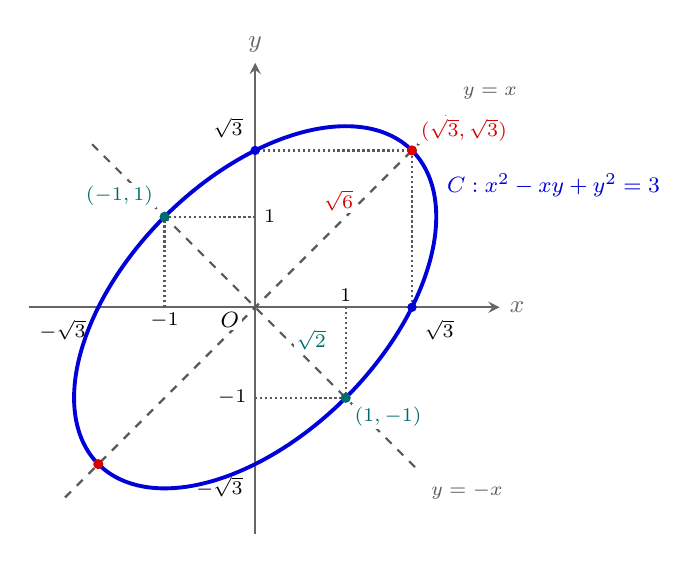
\begin{tikzpicture}[x=1.15cm, y=1.15cm, >=stealth, every node/.style={font=\small}]
    \pgfmathsetmacro{\rThree}{sqrt(3)}
    \coordinate (O) at (0, 0);
    \coordinate (V1) at (\rThree, \rThree);
    \coordinate (V2) at (-\rThree, -\rThree);
    \coordinate (W1) at (-1, 1);
    \coordinate (W2) at (1, -1);

    % 座標軸と対称軸 y = \pm x
    \draw[->, thick, gray!80!black] (-2.5, 0) -- (2.7, 0) node[right] {$x$};
    \draw[->, thick, gray!80!black] (0, -2.5) -- (0, 2.7) node[above] {$y$};

    \draw[dashed, thick, gray!70!black] (-2.1, -2.1) -- (2.15, 2.15)
    node[above right=1pt, font=\scriptsize] {$y=x$};
    \draw[dashed, thick, gray!70!black] (-1.8, 1.8) -- (1.8, -1.8)
    node[below right=1pt, font=\scriptsize] {$y=-x$};
    \node[font=\footnotesize, fill=white, inner sep=1pt] at (-0.28, -0.14) {$O$};

    % 代表点から座標軸への点線垂線
    \draw[densely dotted, thick, gray!70!black] (\rThree, 0) -- (V1) -- (0, \rThree);
    \draw[densely dotted, thick, gray!70!black] (1, 0) -- (W2) -- (0, -1);
    \draw[densely dotted, thick, gray!70!black] (-1, 0) -- (W1) -- (0, 1);

    % 曲線 C: x^2 - xy + y^2 = 3
    \draw[line width=1.4pt, blue!85!black, domain=0:360, samples=120, smooth]
    plot ({\rThree*cos(\x) - sin(\x)}, {\rThree*cos(\x) + sin(\x)});
    \node[blue!85!black, font=\footnotesize, right=2pt] at (1.95, 1.35) {$C:x^2-xy+y^2=3$};

    % 長半径・短半径の注記
    \node[font=\scriptsize, red!85!black, fill=white, inner sep=1pt] at (0.92, 1.18) {$\sqrt{6}$};
    \node[font=\scriptsize, teal!85!black, fill=white, inner sep=1pt] at (0.62, -0.36) {$\sqrt{2}$};

    % 軸上の目盛りと特徴点
    \node[below right=1pt, font=\scriptsize] at (\rThree, 0) {$\sqrt{3}$};
    \node[below left=1pt, font=\scriptsize] at (-\rThree, 0) {$-\sqrt{3}$};
    \node[above left=1pt, font=\scriptsize] at (0, \rThree) {$\sqrt{3}$};
    \node[below left=1pt, font=\scriptsize] at (0, -\rThree) {$-\sqrt{3}$};
    \node[above=1pt, font=\scriptsize, fill=white, inner sep=1pt] at (1, 0) {$1$};
    \node[below=1pt, font=\scriptsize, fill=white, inner sep=1pt] at (-1, 0) {$-1$};
    \node[right=2pt, font=\scriptsize, fill=white, inner sep=1pt] at (0, 1) {$1$};
    \node[left=2pt, font=\scriptsize, fill=white, inner sep=1pt] at (0, -1) {$-1$};

    \node[circle, fill=red!85!black, inner sep=1.3pt] at (V1) {};
    \node[above right=2pt, font=\scriptsize, red!85!black, fill=white, inner sep=1pt] at (V1) {$(\sqrt{3},\sqrt{3})$};
    \node[circle, fill=red!85!black, inner sep=1.3pt] at (V2) {};
    \node[circle, fill=teal!85!black, inner sep=1.3pt] at (W1) {};
    \node[above left=3pt, font=\scriptsize, teal!85!black, fill=white, inner sep=1pt] at (W1) {$(-1,1)$};
    \node[circle, fill=teal!85!black, inner sep=1.3pt] at (W2) {};
    \node[below right=2pt, font=\scriptsize, teal!85!black, fill=white, inner sep=1pt] at (W2) {$(1,-1)$};
    \node[circle, fill=blue!85!black, inner sep=1.2pt] at (\rThree, 0) {};
    \node[circle, fill=blue!85!black, inner sep=1.2pt] at (0, \rThree) {};
  \end{tikzpicture}
  \caption{曲線 $C:x^2-xy+y^2=3$ の概形（長半径 $\sqrt{6}$，短半径 $\sqrt{2}$ の楕円）}
  \label{fig:rotated_ellipse_c}
\end{figure}

また，求める面積$S$は，$C'$側で考えれば下図斜線部である．($x=0$，$y=0$を$\pi/4$回転させると$y=\pm x$に成る．)

\begin{figure}[htb]
  \centering
  \begin{tikzpicture}[scale=1.0, >=stealth, every node/.style={font=\small}]
    % ----------------------------------------------------
    % 左パネル: 楕円 C' (x^2 + 3y^2 = 6) と直線 y = \pm x
    % ----------------------------------------------------
    \begin{scope}[shift={(0, 0)}, scale=0.95]
      \pgfmathsetmacro{\aVal}{sqrt(6)}
      \pgfmathsetmacro{\bVal}{sqrt(2)}
      \pgfmathsetmacro{\xInt}{sqrt(1.5)}

      % 斜線領域 (面積 S)
      \fill[pattern=north east lines, pattern color=blue!60]
      (0, 0) -- (\xInt, \xInt)
      -- plot[domain=60:-60, samples=50, smooth] ({\aVal*cos(\x)}, {\bVal*sin(\x)})
      -- cycle;

      % 座標軸
      \draw[->, thick, gray!80!black] (-2.85, 0) -- (3.1, 0) node[right] {$x$};
      \draw[->, thick, gray!80!black] (0, -2.05) -- (0, 2.25) node[above] {$y$};

      % 楕円 C' と境界直線 y = \pm x
      \draw[line width=1.3pt, blue!85!black, domain=0:360, samples=100, smooth]
      plot ({\aVal*cos(\x)}, {\bVal*sin(\x)});
      \node[blue!85!black, font=\scriptsize, above left=1pt] at (-1.55, 1.1) {$C':x^2+3y^2=6$};

      \draw[line width=1.1pt, teal!85!black] (-1.55, -1.55) -- (1.85, 1.85)
      node[above right=1pt, font=\scriptsize] {$y=x$};
      \draw[line width=1.1pt, teal!85!black] (-1.55, 1.55) -- (1.85, -1.85)
      node[below right=1pt, font=\scriptsize] {$y=-x$};
      \node[font=\scriptsize, fill=white, inner sep=1pt] at (-0.36, -0.15) {$O$};

      % 交点からの垂線と軸ラベル
      \draw[densely dotted, thick, gray!70!black] (\xInt, -\xInt) -- (\xInt, \xInt);
      \node[below=2pt, font=\scriptsize, fill=white, inner sep=1pt] at (\xInt, 0) {$\frac{\sqrt{6}}{2}$};
      \node[below right=1pt, font=\scriptsize] at (\aVal, 0) {$\sqrt{6}$};
      \node[below left=1pt, font=\scriptsize] at (-\aVal, 0) {$-\sqrt{6}$};
      \node[above left=1pt, font=\scriptsize] at (0, \bVal) {$\sqrt{2}$};
      \node[below left=1pt, font=\scriptsize] at (0, -\bVal) {$-\sqrt{2}$};

      \node[circle, fill=red!85!black, inner sep=1.3pt] at (\xInt, \xInt) {};
      \node[circle, fill=red!85!black, inner sep=1.3pt] at (\xInt, -\xInt) {};
      \node[font=\footnotesize, fill=white, inner sep=1.5pt] at (1.65, 0.32) {$S$};
      \node[below, font=\footnotesize] at (0.1, -2.3) {$C'$ 上での対応領域};
    \end{scope}

    % ----------------------------------------------------
    % 右パネル: 伸縮変換 (X, Y) = (x/\sqrt{6}, y/\sqrt{2}) 後の単位円
    % ----------------------------------------------------
    \begin{scope}[shift={(6.4, 0)}, scale=1.45]
      \pgfmathsetmacro{\yHalf}{sqrt(3)/2}

      % 扇形領域 (中心角 2\pi/3)
      \fill[pattern=north east lines, pattern color=blue!60]
      (0, 0) -- (60:1) arc[start angle=60, end angle=-60, radius=1] -- cycle;

      % 座標軸
      \draw[->, thick, gray!80!black] (-1.35, 0) -- (1.55, 0) node[right] {$X$};
      \draw[->, thick, gray!80!black] (0, -1.4) -- (0, 1.55) node[above] {$Y$};
      \node[below left=2pt] at (0, 0) {$O$};

      % 単位円と直線 Y = \pm \sqrt{3} X
      \draw[line width=1.3pt, blue!85!black] (0, 0) circle (1);
      \draw[line width=1.1pt, teal!85!black] (-0.68, {-0.68*sqrt(3)}) -- (0.76, {0.76*sqrt(3)})
      node[above right=1pt, font=\scriptsize] {$Y=\sqrt{3}X$};
      \draw[line width=1.1pt, teal!85!black] (-0.68, {0.68*sqrt(3)}) -- (0.76, {-0.76*sqrt(3)})
      node[below right=1pt, font=\scriptsize] {$Y=-\sqrt{3}X$};

      % 中心角 \pi/3 と交点垂線
      \draw[thick, red!85!black] (0.36, 0) arc[start angle=0, end angle=60, radius=0.36];
      \node[font=\scriptsize, red!85!black, fill=white, inner sep=1pt] at (30:0.53) {$\frac{\pi}{3}$};

      \draw[densely dotted, thick, gray!70!black] (0.5, 0) -- (0.5, \yHalf) -- (0, \yHalf);
      \node[below=2pt, font=\scriptsize, fill=white, inner sep=1pt] at (0.5, 0) {$\frac{1}{2}$};
      \node[left=2pt, font=\scriptsize, fill=white, inner sep=1pt] at (0, \yHalf) {$\frac{\sqrt{3}}{2}$};
      \node[below right=1pt, font=\scriptsize] at (1, 0) {$1$};
      \node[above left=1pt, font=\scriptsize] at (0, 1) {$1$};

      \node[circle, fill=red!85!black, inner sep=1.3pt] at (0.5, \yHalf) {};
      \node[circle, fill=red!85!black, inner sep=1.3pt] at (0.5, -\yHalf) {};
      \node[below, font=\footnotesize] at (0.1, -1.62) {座標変換後の扇形};
    \end{scope}
  \end{tikzpicture}
  \caption{回転後の楕円 $C'$ における斜線部（左）と座標変換 $(X,Y)=(x/\sqrt{6},\,y/\sqrt{2})$ 後の単位円の扇形（右）}
  \label{fig:ellipse_to_sector}
\end{figure}

ここで$(X,Y)=(x/\sqrt{6},y/\sqrt{2})$なる座標変換をすると，右上図のようになるから，
\begin{align}
  \dfrac{1}{\sqrt{6}}\dfrac{1}{\sqrt{2}}S=\dfrac{1}{2}\dfrac{2\pi}{3} \\
  S=\dfrac{2\sqrt{3}\pi}{3}
\end{align}
である．$\cdots$(答)

\newpage
\end{document}
